% Copyright (c) 2015 Benito Palacios Sánchez - All Rights Reserved.
% Esta obra está licenciada bajo la Licencia Creative Commons Atribución 4.0
% Internacional. Para ver una copia de esta licencia, visita
% http://creativecommons.org/licenses/by/4.0/.

\section{Servicios en línea}
\subsection{Multijugador}
\begin{frame}[fragile]{Captura de paquetes}
\begin{columns}

\begin{column}{0.35\textwidth}
Estrategia \textit{man-in-the-middle}
\begin{center}
    \includefigure{\textit{Man-in-the-middle}}{imgs/man_middle.eps}
\end{center}
\end{column}

\begin{column}{0.5\textwidth}
\uncover<2->{Modificación DeSmuME.}
\begin{itemize}
    \item<3-> Paquetes PCAP.
\end{itemize}
\begin{uncoverenv}<3->\begin{lstlisting}
void create_packet();
void save_packet(u8* packet,u32 len);
void save_adhocPacket(u8* packet,
  u32 len, void* addr, bool isSent);
\end{lstlisting}\end{uncoverenv}

\begin{itemize}
    \item<4-> Exportar paquetes.
\end{itemize}
\uncover<5->{\scriptsize\texttt{HandleDebugEvent\_Execute()} en \texttt{debug.cpp}.}
\vfill
\visible<6->{\includefigure{\textit{RC4Finder.}}{imgs/rc4finder.png}}
\end{column}

\end{columns}
\end{frame}

\begin{frame}{Servidores para Nintendo DS}

\begin{center}
    \visible<2->{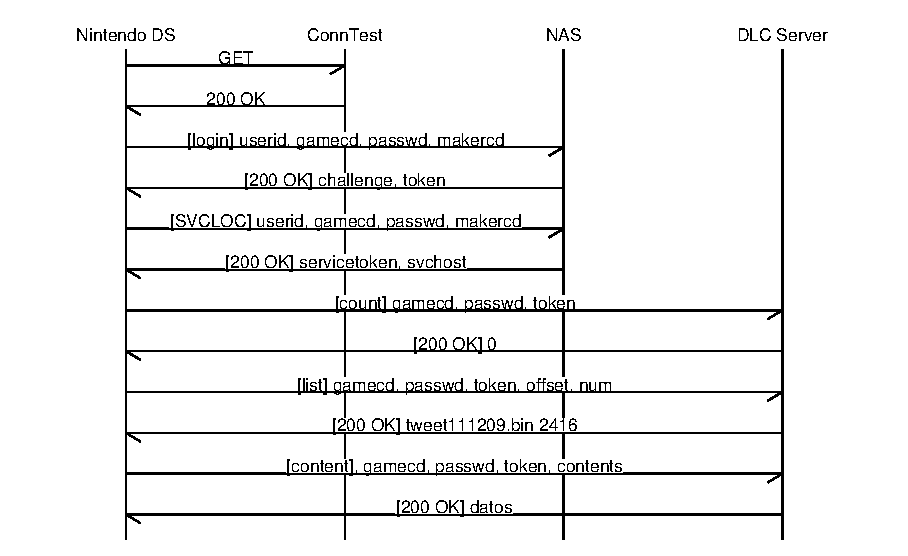
\includegraphics[width=\textwidth,height=0.5\textheight,keepaspectratio]{imgs/nds_dwc.eps}}
\end{center}

\uncover<3->{Vulnerabilidades:}
\begin{columns}
\footnotesize
\begin{column}{0.3333\textwidth}
    \begin{itemize}
        \item<4-> Puerto 80 del NAS abierto.
    \end{itemize}
\end{column}
\begin{column}{0.3333\textwidth}
    \begin{itemize}
        \item<5-> Contraseña no usada.
    \end{itemize}
\end{column}
\begin{column}{0.3333\textwidth}
    \begin{itemize}
        \item<6-> Autenticación simple.
    \end{itemize}
\end{column}

\end{columns}
\end{frame}

\begin{frame}{Preguntados}
\begin{columns}
    \begin{column}{0.15\textwidth}
        
\includegraphics[width=\textwidth,keepaspectratio]{imgs/preguntados_logo.png}
    \end{column}
    \begin{column}{0.85\textwidth}
        Trivial para plataformas móviles.
    \end{column}
\end{columns}

\vfill
\vspace{0.35cm}
\uncover<2->{Vulnerabilidades:}
\begin{columns}
    \begin{column}{0.5\textwidth}
    \begin{itemize}
        \item<3-> Comunicación HTTP.
    \end{itemize}
    \end{column}

    \begin{column}{0.5\textwidth}
    \begin{itemize}
        \item<4-> Solución enviada antes de preguntar.
    \end{itemize}
    \end{column}
\end{columns}

\only<4>{\includefigure{Preguntas, respuesta y solución de una partida}{imgs/preguntados_hack.png}}

\only<5>{\includefigure{Preguntas, respuesta y solución de una partida}{imgs/preguntados_hack_question.png}}

\only<6>{\includefigure{Preguntas, respuesta y solución de una partida}{imgs/preguntados_hack_answer.png}}

\end{frame}

\subsection{Contenidos descargables}
\begin{frame}{Duet}
\begin{center}
\includegraphics[width=0.15\textwidth,keepaspectratio]{imgs/duet_logo.png}\end{center}

\begin{columns}
    \begin{column}{0.5\textwidth}
    \begin{itemize}
        \item<2-> Niveles extras por 0,99€.
        \item<4-> BD con preferencias sin proteger.
        \note<1>[item]{Es SQLite y se puede usar software como SQLiteMan}
    \end{itemize}
    \end{column}

    \begin{column}{0.5\textwidth}
    \begin{itemize}
        \item<3-> Ya incluidos pero desactivados.
        \item<5-> Se puede activar a mano.
    \end{itemize}
    \end{column}
\end{columns}

\visible<5->{\includefigure{Filas con estado de los contenidos extras}{imgs/duet-levels.png}}

\end{frame}

\begin{frame}{\textit{Download Play}}
Compartir demos con comunicación inalámbrica ad-hoc.
\vfill
\uncover<2->{\underline{Problema:}}
\begin{itemize}
    \item<3-> Envío de código de una consola a otra.
    \item<4-> El código principales se firman con \texttt{RSA}.
\end{itemize}
\vfill
\uncover<5->{\underline{Solución de Nintendo:}}
\begin{itemize}
    \item<6-> Comprobar integridad con \texttt{HMAC}.
    \item<7-> Solo si con \textit{Download Play}.
\end{itemize}
\end{frame}
